\documentclass{beamer}
\usetheme{Montpellier}
\usecolortheme{beaver}
\usepackage{verbatim}	
\usepackage[square,sort]{natbib}
\usepackage{comment}
\usepackage{amsmath}
\usepackage{caption}
\usepackage{diagbox}
\usepackage{xcolor}
\usepackage{booktabs}

\setbeamerfont{footnote}{size=\tiny}
\setbeamerfont{footnote mark}{size=\tiny}
\setbeamerfont{caption}{size=\scriptsize}
\setbeamerfont{cite}{size=\tiny}

\title{PIRT - Parallel Iterative Reconstruction Tomography, with center of rotation error correction}

\author{Team : Sajid Ali \textsuperscript{1}, Panpan Huang \textsuperscript{1}, Zichao Wendy Di \textsuperscript{2} \newline \newline Mentors : Barry Smith \textsuperscript{2} \& Hong Zhang \textsuperscript{2} }
\institute[shortinst]{\textsuperscript{1} Northwestern University \and \inst{2} Argonne National Laboratory}

\date{Argonne GPU Hackathon 2021}

\begin{document}

%\begin{frame}
%\titlepage
%\end{frame}

\begin{frame}
\begin{center}
	\begin{figure}
		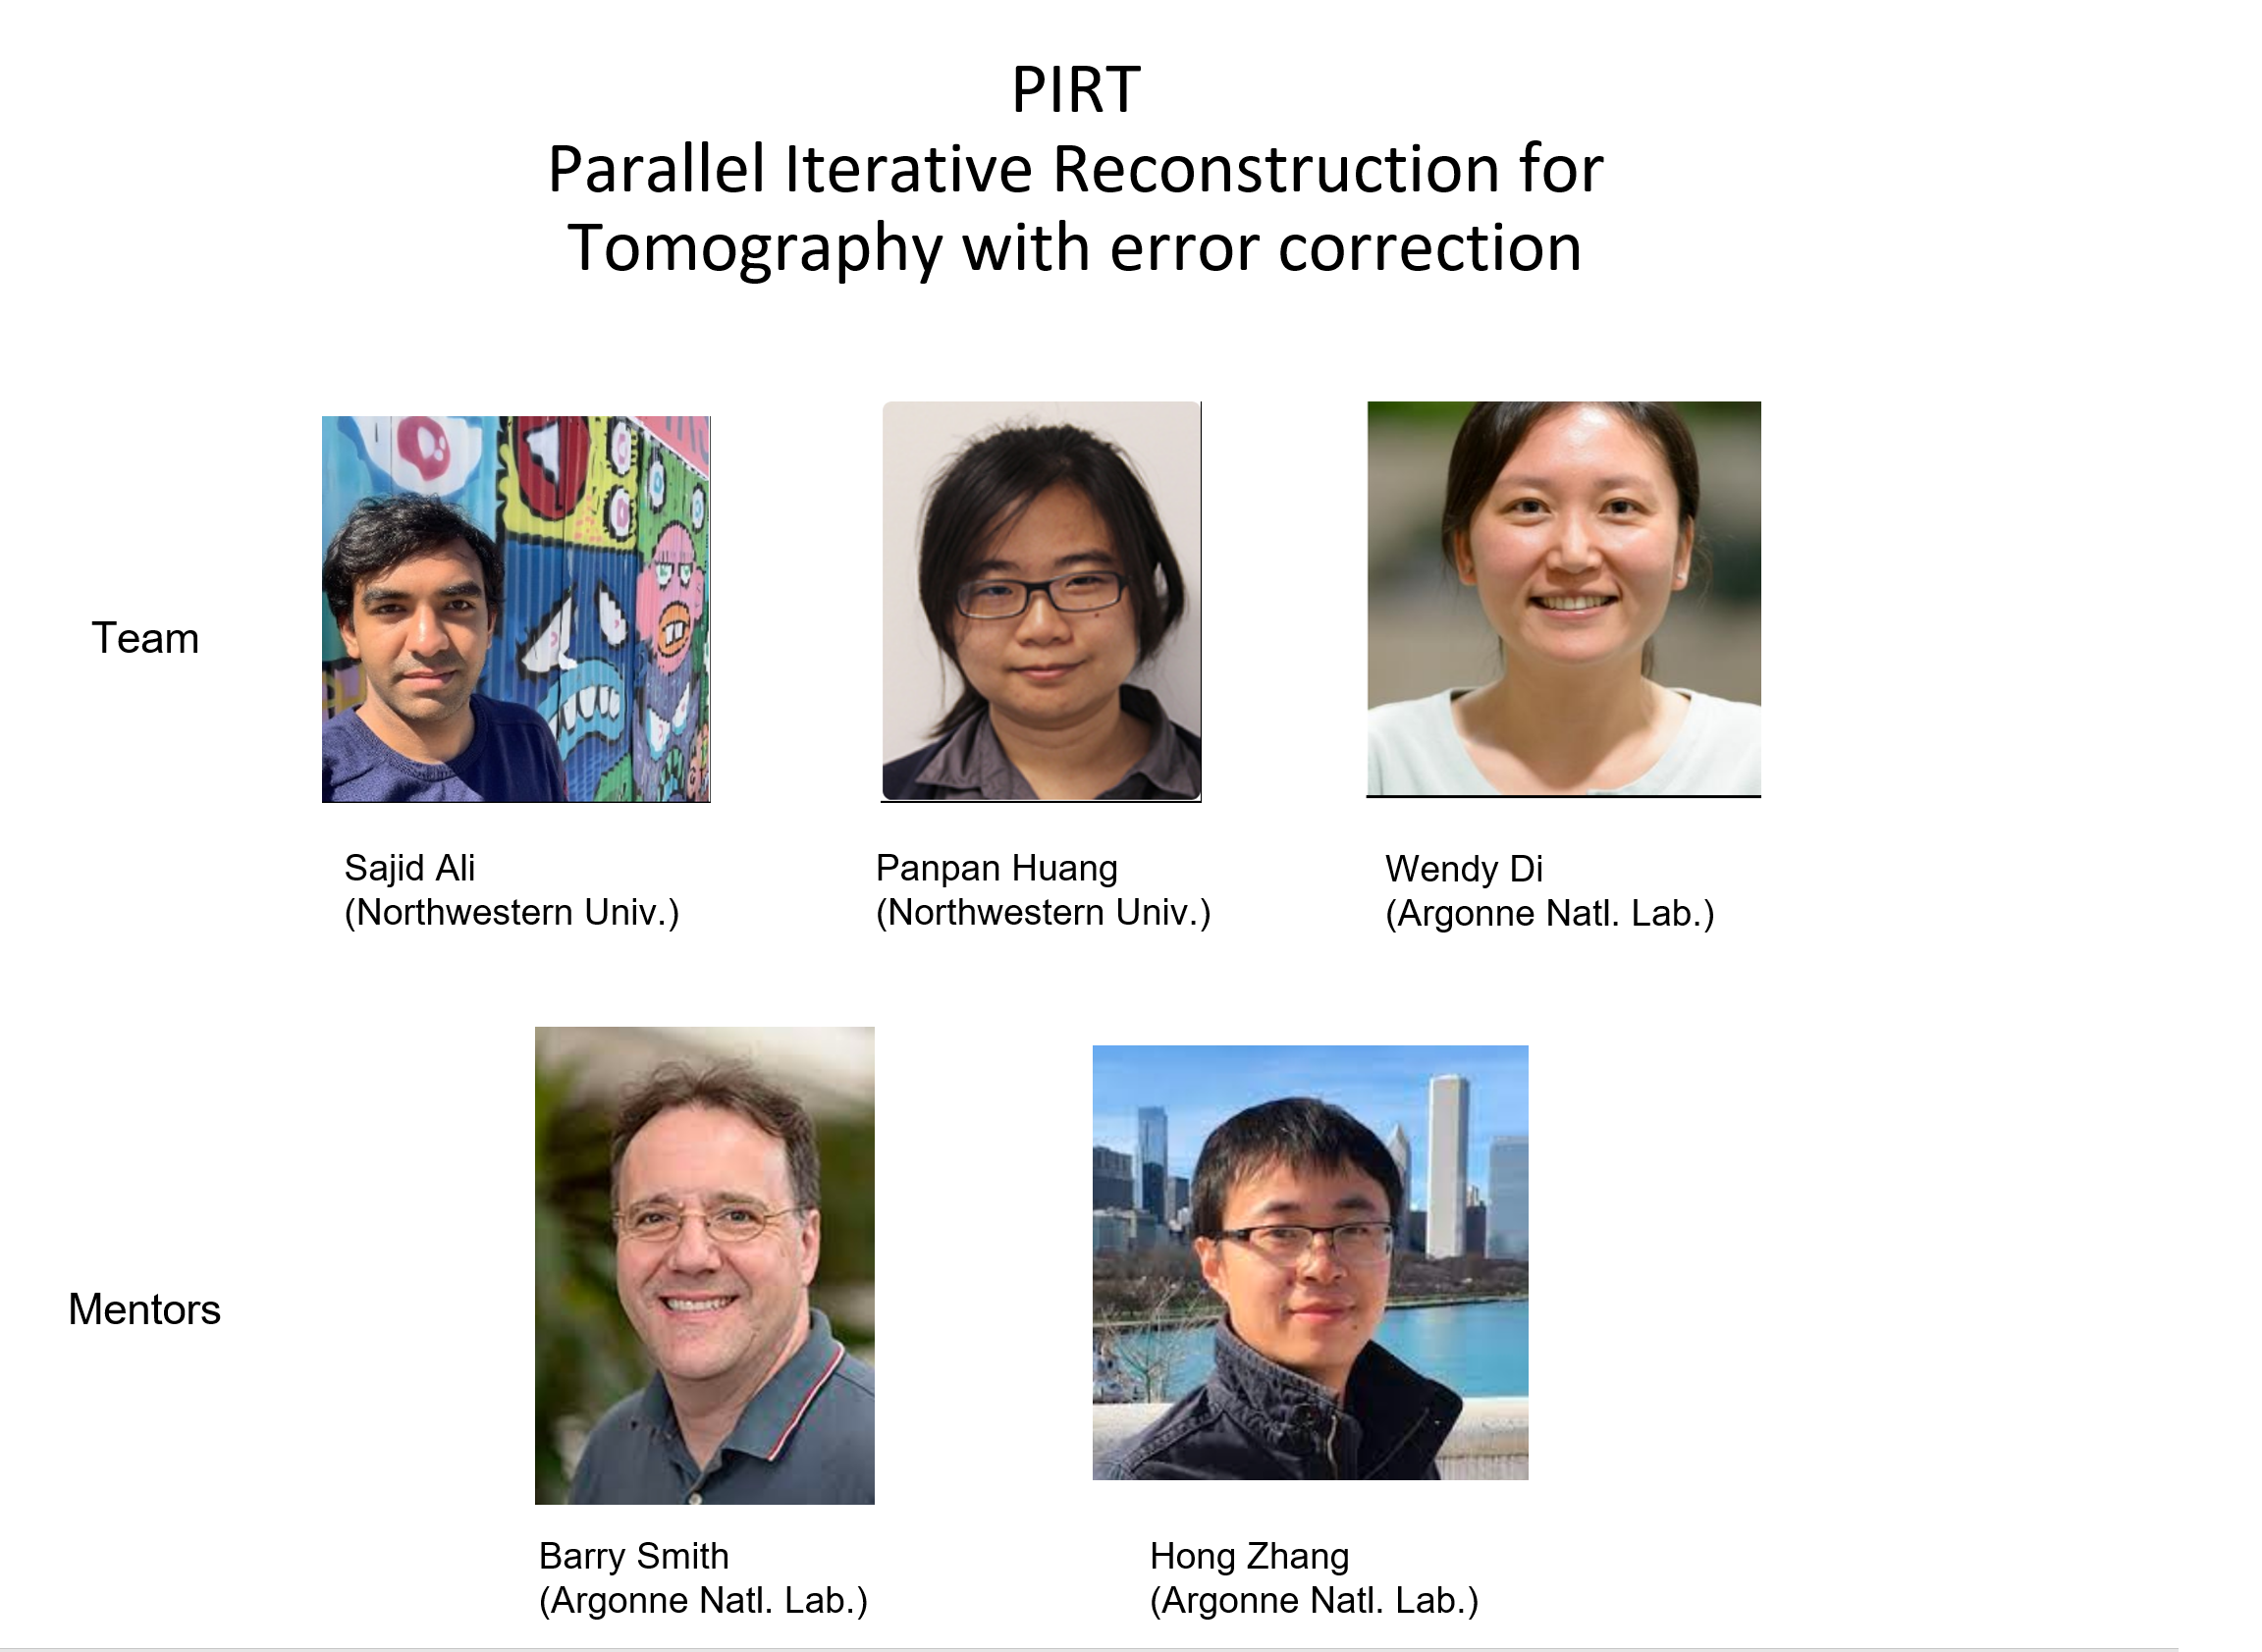
\includegraphics[scale=0.25]{figures/pirt}
	\end{figure}
\end{center}
\end{frame}


\section{Application}

\begin{frame}{Optimization formulation}
	\begin{block}{Least squares cost function for tomography inversion, with error correction}
		\begin{itemize}
			%\item Assuming no shifts, we need
			%$\underset{\mathcal{W} \geq 0}{\textit{min}}  %\frac{1}{2}||\mathcal{L}\mathcal{W}-\mathcal{D}||$
			\item To recover both shifts and object : 
			$\underset{\mathcal{W} \geq 0, P_{\theta}}{\textit{min}}  \phi(\mathcal{W},P_{\theta}) = \frac{1}{2}||\mathcal{L}\mathcal{W} - g(\mathcal{D},P_{\theta})||$
			\item First order derivatives analytically computable :
			$ \nabla \phi(\mathcal{W},P_{\theta}) = [\mathcal{L}^{T},
			\nabla_{P_{\theta}} \phi(\mathcal{W},P_{\theta})]^{T} (\mathcal{L}\mathcal{W} - g(\mathcal{D},P_{\theta}))$
		\end{itemize}
	\end{block}
	\begin{exampleblock}{Varaits}
	\begin{itemize}
		\item Joint : Combine shifts and sample into one vector and optimize for both together.
		\item Alternating : Alternate between optimizing with respect to sample and with respect to shifts.
	\end{itemize}
	\end{exampleblock}
\end{frame}
\begin{frame}{Implementation}
	\begin{block}{Language / Libraries / Architecture}
		\begin{itemize}
			\item C/C++ using the PETSc/TAO framework
			\item Boost-geometry for the setup phase ($<2\%$ of runtime) 
			\item FFTW for (MPI-rank local) fourier space convolutions
			\item 2-level MPI parallelism : MPI subcommunicators for concurrent instances of solver, each of which runs a TAO optimization problem with occasional syncing via PETSc VecScatters.
			\item Owing to the performance portable nature of PETSc, the non-error correcting version already runs on GPU's!
		\end{itemize}
	\end{block}
\end{frame}

\section{Evolution and Strategy}
\begin{frame}{Port Path \& Goals }
	\begin{block}{GPU Port path : }
		\begin{itemize}
			\item FFTW $\rightarrow$ cuFFT 
			\item CUB for block-wise reductions
			\item remaining $for$ loops $\rightarrow$ CUDA kernels
		\end{itemize}
	\end{block}
    \begin{exampleblock}{Goals}
	  \begin{itemize}
		\item Focus on porting the TAO objective function $\&$ gradient routines in addition to some helper routines.
		\item Profile GPU versions to ensure that the port is efficient.
		\item If the single slice, single instance solver works, begin investigation of running concurrent solver instances.
      \end{itemize}
    \end{exampleblock}
\end{frame}

\begin{frame}{Change in strategy}
  \begin{block}{Surprises!}
	\begin{itemize}
		\item Typically, $>90\%$ of total time is spent in objective function/gradient routines, but on theta-gpu, $<5\%$.
		\item Bottleneck : setting up non-contiguous data transfers between GPU arrays for bounds projection from estimated active set.
    \end{itemize}
  \end{block}	
  \begin{exampleblock}{Alternatives to explore}
    \begin{itemize}
      \item Remove bound constraints $\rightarrow$ solution quality degrades.
      \item Re-evaluate for problem sizes of interest to APS beamlines ?
      \item If the active-set estimation/bound projection bottleneck still exists, explore alternate formulations like Augmented Lagrangian multiplier method.
   \end{itemize}
  \end{exampleblock}
\end{frame}

\section{Results and Final Profile}
\begin{frame}{Results and Final Profile}
\begin{table}[]
	\centering
	\scalebox{0.85}{
	\begin{tabular}{lllllllll}
		\toprule
		& \multicolumn{2}{l}{1 MPI Rank} & \multicolumn{2}{l}{4 MPI ranks} & \multicolumn{2}{l}{8 MPI Ranks} & \multicolumn{2}{l}{16 MPI Ranks} \\ 
		& Total     & \% f/g    & Total     & \% f/g    & Total     & \% f/g    & Total     & \% f/g     \\ \midrule
		
		\textcolor{cyan}{CPU-joint} & 899.0 & \textcolor{cyan}{89.7} & 250.2 & \textcolor{cyan}{84.1} & 134.4 & \textcolor{cyan}{84.8} & 79.0 & \textcolor{cyan}{86.5}     \\
		
		\textcolor{magenta}{GPU-joint} & 128.8     & \textcolor{magenta}{2.9}  & 66.2      & \textcolor{magenta}{5.8} & 37.8      & \textcolor{magenta}{12.4}      & 58.9      & \textcolor{magenta}{21.3}       \\ \midrule
		
		\textcolor{cyan}{CPU-alt}   & 765.9     & \textcolor{cyan}{97.6}      & 185.8     & \textcolor{cyan}{96.4}      & 100.4     & \textcolor{cyan}{96.5}      & 58.8      & \textcolor{cyan}{96.8}       \\
		
		\textcolor{magenta}{GPU-alt}  & 22.5      & \textcolor{magenta}{12.7}      & 11.8      & \textcolor{magenta}{17.4}      & 9.5       & \textcolor{magenta}{30.0}      & 22.4      & \textcolor{magenta}{54.1}       \\ 
	    \bottomrule
	\end{tabular}
    }
    \caption{\label{tab:table-name}Analysis of total time as a function of MPI ranks for CPU and GPU solves and $\%$ of time spent in evaluation objective function and gradient.}
\end{table}
\end{frame}

\section{Problems encountered \& Wishlist} 
\begin{frame}{Problems encountered \& Wishlist}
  \begin{block}{Problems encountered}
  	\begin{itemize}
	  \item Some problems with using nvhpc which went away when using gcc and cuda with spack directly.
    \end{itemize}
  \end{block}	
  \begin{exampleblock}{Wishlist}
	\begin{itemize}
		\item Better integration of nvhpc compiler within spack.
	\end{itemize}
  \end{exampleblock}		
\end{frame}

\section{Was it worth it ?} 
\begin{frame}{Was it worth it ?} 
	\begin{itemize}
	\item Emphatic Yes! Presence of library developers and tool experts eased the path to porting and analyzing application. This, coupled with access to the latest generation GPU compute nodes helped in generating an informal performance model.
	\item We will follow up by taking a decision on the path forward for the application in terms of algorithm choice.
	\item  	\textcolor{teal}{Thank you to all the organizers for putting this event together and to both our mentors for all the advice and help in porting our application!}
	\end{itemize}	
	
\end{frame}

\renewcommand*{\bibfont}{\scriptsize}
\begin{frame}[t, allowframebreaks]
	\frametitle{References}
	\bibliographystyle{dinat-etal}
	\bibliography{pirt}
\end{frame}

\end{document}
